% !TeX spellcheck = pt_BR
%%%%%%%%%%%%%%%%%%%%%%%%%%%%%%%%%%%%%%%%%
% Beamer Presentation
% LaTeX Template
% Version 1.0 (10/11/12)
%
% Updated by Felipe Timóteo | felipetimote@id.uff.br
% (28/01/2019) 
% This template has been downloaded from:
% http://www.LaTeXTemplates.com
%
% License:
% CC BY-NC-SA 3.0 (http://creativecommons.org/licenses/by-nc-sa/3.0/)
%
%%%%%%%%%%%%%%%%%%%%%%%%%%%%%%%%%%%%%%%%%

%----------------------------------------------------------------------------------------
%	PACKAGES AND THEMES
%----------------------------------------------------------------------------------------

\documentclass[xcolor=dvipsnames,t]{beamer}
% The Beamer class comes with a number of default slide themes
% which change the colors and layouts of slides. Below this is a list
% of all the themes, uncomment each in turn to see what they look like.

%\usetheme{default}
%\usetheme{AnnArbor}
%\usetheme{Antibes}
%\usetheme{Bergen}
%\usetheme{Berkeley}
%\usetheme{Berlin}
\usetheme{Boadilla}
%\usetheme{CambridgeUS}
%\usetheme{Copenhagen}
%\usetheme{Darmstadt}
%\usetheme{Dresden}
%\usetheme{Frankfurt}
%\usetheme{Goettingen}
%\usetheme{Hannover}
%\usetheme{Ilmenau}
%\usetheme{JuanLesPins}
%\usetheme{Luebeck}
%\usetheme{Madrid}
%\usetheme{Malmoe}
%\usetheme{Marburg}
%\usetheme{Montpellier}
%\usetheme{PaloAlto}
%\usetheme{Pittsburgh}
%\usetheme{Rochester}
%\usetheme{Singapore}
%\usetheme{Szeged}
%\usetheme{Warsaw}


% As well as themes, the Beamer class has a number of color themes
% for any slide theme. Uncomment each of these in turn to see how it
% changes the colors of your current slide theme.

%\usecolortheme{albatross}
%\usecolortheme{beaver}
%\usecolortheme{beetle}
%\usecolortheme{crane}
%\usecolortheme{dolphin}
%\usecolortheme{dove}
%\usecolortheme{fly}
%\usecolortheme{lily}
%\usecolortheme{orchid}
\usecolortheme{rose}
%\usecolortheme{seagull}
%\usecolortheme{seahorse}
%\usecolortheme{whale}
%\usecolortheme{wolverine}
%\usecolortheme[named=Maroon]{structure} % customize theme color
%}

% ---
% PACOTES
% ---
\usepackage[alf]{abntex2cite}		% Citações padrão ABNT
%\usepackage[brazil]{babel}		% Idioma do documento
\usepackage[english]{babel}		% Idioma do documento
\usepackage{color}			% Controle das cores
\usepackage[T1]{fontenc}		% Selecao de codigos de fonte.
\usepackage{graphicx}			% Inclusão de gráficos
\usepackage[utf8]{inputenc}		% Codificacao do documento (conversão automática dos acentos)
\usepackage{txfonts}			% Fontes virtuais


\usepackage{xcolor}
\usepackage{graphicx}
%\usepackage{MnSymbol}
\usepackage{stmaryrd}
\usepackage{colortbl}
\usepackage{caption}
\usepackage{comment}
\usepackage{pdfpages}
\usepackage{booktabs}
\usepackage{soul}
\usepackage[normalem]{ulem}
\usepackage{amsmath}
\usepackage{tcolorbox}
%\usepackage{lipsum}

%%%%%%%%%%%%%%%%%%%%%%%%%%%%%%%%%%%%%%%%%%%%%%%%%
\usepackage{pgf}
%\usepackage{etex}
%\usepackage{tikz,pgfplots}
\usepackage{tikz}
\usepackage{bm}                 % letras gregas em negrito
\usepackage{cancel}             % goes to zero 
\usepackage{amsmath}            % usado para criar subequações

\usepackage{hyperref}          % hyperlink
\usefonttheme{professionalfonts}

\useoutertheme{infolines}
%\useoutertheme{miniframes}
%\useoutertheme{shadow}
%\useoutertheme{sidebar}
%\useoutertheme{smoothbars}
%\useoutertheme{smoothtree}
%\useoutertheme{split}
%\useoutertheme{tree}

%\useinnertheme{default}
%\useinnertheme{circles}
%\useinnertheme{rectangles}


%%%%%%%%%%%%%%%%%%%%%%%%%%%%%%%%%%%%%%%%%%%%%%%%%
%multiinclude
%\usepackage{xmpmulti}

\usepackage{subfig} % Written by Steven Douglas Cochran
% This package makes it easy to put subfigures
%%%% in your figures. i.e., "figure 1a and 1b"
% Docs are in "Using Imported Graphics in LaTeX2e"
% by Keith Reckdahl which also documents the graphicx
% package (see above). subfigure.sty is already
% installed on most LaTeX systems. The latest version
% and documentation can be obtained at:
% http://www.ctan.org/tex-archive/macros/latex/contrib/supported/subfigure/


%%%%%%%%%%%%%%%%%%%%%%%%%%%%%%%%%%%%%%%%%%%%%%%%%
\usepackage{listings}     %used to write code
\newcommand{\estiloJava}{
	\lstset{
		language=Java,
		basicstyle=\ttfamily\small,
		keywordstyle=\color{jpurple}\bfseries,
		stringstyle=\color{red},
		commentstyle=\color{verde},
		morecomment=[s][\color{blue}]{/**}{*/},
		extendedchars=true,
		showspaces=false,
		showstringspaces=false,
		numbers=left,
		numberstyle=\tiny,
		breaklines=true,
		backgroundcolor=\color{cyan!10},
		breakautoindent=true,
		captionpos=b,
		xleftmargin=0pt,
		tabsize=2
	}}

\usepackage{color}
\usepackage[ruled,vlined]{algorithm2e}  %used to pseudo code - algorithms

%%%%%%%%%%%%%%%%%%%%%%%%%%%%%%%%%%%%%%%%%%%%%%%%%%
% Tcolorbox
\newtcolorbox{mybox}[2][]{colback=red!5!white,colframe=red!75!black,fonttitle=\bfseries, 	colbacktitle=red!85!black, enhanced, attach boxed title to top center={yshift=-2mm},title=#2,#1}


%%%%%%%%%%%%%%%%%%%%%%%%%%%%%%%%%%%%%%%%%%%%%%%%%%
% Some Configurations
\setbeamertemplate{caption}[numbered]        % Numbering figures
\setbeamertemplate{bibliography item}[book]  % Remove icons from bibliography

\definecolor{dkgreen}{rgb}{0,0.6,0}
\definecolor{gray}{rgb}{0.5,0.5,0.5}
\definecolor{mauve}{rgb}{0.58,0,0.82}

\lstset{frame=tb,
  language=Java,
  aboveskip=2mm,
  belowskip=2mm,
  showstringspaces=false,
  columns=flexible,
  basicstyle={\small\ttfamily},
  numbers=none,
  numberstyle=\tiny\color{gray},
  keywordstyle=\color{blue},
  commentstyle=\color{dkgreen},
  stringstyle=\color{mauve},
  breaklines=true,
  breakatwhitespace=true,
  tabsize=2
}

%%%%%%%%%%%%%%%%%%%%%%%%%%%%%%%%%%%%%%%%%%%%%%%%%
\title[Git]{Controle de Versão e Introdução 
\includegraphics[height=0.35cm]{figures/gitlogo.png}}

\author[@fetim]{Felipe Timóteo}
\institute{GISIS \& DOT-UFF }
\date{\today}
\logo{\pgfimage[height=1.0cm]{figures/0_logo.pdf}}
\titlegraphic{
\includegraphics[height=2.5cm]{figures/1_logo.pdf}}

\begin{document}

% ----------------- NOVO SLIDE --------------------------------	
\begin{frame}
  \titlepage
\end{frame}

\setbeamertemplate{enumerate items}[circle]
\setbeamertemplate{section in toc}[square]
\setbeamertemplate{subsection in toc}[square]
% ----------------- NOVO SLIDE --------------------------------	
\begin{frame}{Outline}
	\tiny
	\tableofcontents%[pausesections]
\end{frame}

\section{Introdução}
% ----------------- NOVO SLIDE --------------------------------	
\begin{frame}{Outline}
\tiny
\tableofcontents[current]
\end{frame}

\subsection{Motivação}
% ----------------- NOVO SLIDE --------------------------------	
\begin{frame}{Introdução}
\framesubtitle{Motivação}
\setbeamercovered{transparent}

\begin{itemize}[<+->]
	\item[$ \checkmark $] Ajuda na organização do projeto de forma eficiente
	\item[$ \checkmark $] Documentação e histórico do desenvolvimento mais robusta
	\item[$ \checkmark $] Facilita a colaboração de pequenos ou grandes grupos
	\item[$ \checkmark $] Economia de tempo durante o desenvolvimento
	\item[$ \checkmark $] Facilita debug de programas complexos
	\item[$ \checkmark $] Muito popular entre os desenvolvedores de softwares
	\item[$ \checkmark $] Evita problemas comum aos desenvolvedores (ou escritores)
	\item[$ \checkmark $] Evita as várias versões diferentes durante a etapa de desenvolvimento
	\item[$ \checkmark $] Evita tarefas chatas e repetitivas
\end{itemize}
\end{frame}


\subsection{Controle de versão}
% ----------------- NOVO SLIDE --------------------------------	
\begin{frame}{Introdução}
\framesubtitle{Controle de versão | fonte: \href{https://guides.github.com/introduction/git-handbook/}{\color{blue} git handbook}}
What’s a version control system?

A \textbf{version control system}, or VCS, \textbf{tracks the history of changes} as people and teams \textbf{collaborate} on projects together. As the project evolves, teams can run tests, fix bugs, and contribute new code with the \textbf{confidence that any version can be recovered at any time}. Developers can \textbf{review project history} to find out:

\begin{itemize}
	\item[$ \bullet $] Which changes were made?
	\item[$ \bullet $] Who made the changes?
	\item[$ \bullet $] When were the changes made?
	\item[$ \bullet $] Why were changes needed?
\end{itemize}

\end{frame}

% ----------------- NOVO SLIDE --------------------------------	
\begin{frame}{Introdução}
\framesubtitle{Controle de versão | fonte: \href{https://guides.github.com/introduction/git-handbook/}{\color{blue} git handbook}}
\small

\begin{exampleblock}{What’s a distributed version control system?}
	Git is an example of a \textbf{distributed version control system} (DVCS) commonly used for open source and commercial software development. DVCSs \textbf{allow full access} to every file, branch, and iteration of a project, and allows every user access to a full and self-contained history of all changes. Unlike once popular \textit{centralized version control systems}, DVCSs like Git don’t need a constant connection to a central repository. Developers can work \textbf{anywhere} and \textbf{collaborate} asynchronously from \textbf{any time} zone
\end{exampleblock}

\begin{block}{}
	Without version control, team members are \textit{subject to redundant tasks, slower timelines, and multiple copies} of a single project. To \textbf{eliminate unnecessary work}, Git and other VCSs give each contributor a unified and consistent view of a project, surfacing work that’s already in progress. Seeing a \textbf{transparent history of changes}, who made them, and how they contribute to the development of a project helps team members stay aligned while working independently.
\end{block}

\end{frame}


\subsection{git}

% ----------------- NOVO SLIDE --------------------------------	
\begin{frame}{Introdução}
\framesubtitle{Why Git? | fonte: \href{https://guides.github.com/introduction/git-handbook/}{\color{blue} git handbook}}
\small
According to the latest Stack Overflow developer survey, more than \textbf{70 percent of developers use Git}, making it the most-used VCS in the world. Git is commonly used for both \textbf{open source} and commercial software development, with significant \textbf{benefits for individuals, teams and businesses}.

\begin{itemize}
	\item[$ \bullet $] Git lets developers \textbf{see the entire timeline} of their changes, decisions, and progression of any project in one place. From the moment they access the history of a project, the developer has all the context they need to understand it and start \textbf{contributing}.
	\item[$ \bullet $] Developers work in every time zone. With a DVCS like Git, collaboration can happen any time while \textbf{maintaining source code integrity}. Using branches, developers can \textbf{safely propose changes to production code}.
	\item[$ \bullet $] Businesses using Git can \textbf{break down communication barriers} between teams and keep them focused on doing their best work. Plus, Git makes it possible to align experts across a business to collaborate on major projects.
\end{itemize}

\end{frame}

\subsection{github \& gitlab}
% ----------------- NOVO SLIDE --------------------------------	
\begin{frame}{Introdução}
\framesubtitle{git | github ou gitlab}

\vfill
\begin{figure}
	\centering
	
\includegraphics[width=0.2\linewidth]{figures/gitlogo.png}
\end{figure}
\vfill
\begin{columns}[t]
	\begin{column}{.5\textwidth}
\begin{figure}
	\centering
	\includegraphics[width=0.7\linewidth]{figures/Github_logo}
\end{figure}
	\end{column}
	\begin{column}{.5\textwidth}
\begin{figure}
	\centering
	
\includegraphics[width=0.7\linewidth]{figures/GitLab_logo}
\end{figure}
	\end{column}
\end{columns}
\vfill

\end{frame}

\section{Git Workflow Básico}

% ----------------- NOVO SLIDE --------------------------------	
\begin{frame}{}
	\tiny
	\tableofcontents[current]
\end{frame}

\subsection{Configurando o git}
% ----------------- NOVO SLIDE --------------------------------	
\begin{frame}[fragile]{Git Workflow}
	\framesubtitle{Preparando o ambiente pela 1ª vez}

	\begin{block}{Defina o user name}		
		\begin{verbatim}
			$ git config --global user.name "[nome]"
		\end{verbatim}
	\end{block}
	
	\begin{block}{Defina o email}
		\begin{verbatim}
			$ git config --global user.email "[endereço-de-email]"
		\end{verbatim}
	\end{block}

	\begin{exampleblock}{Melhore a visualização usando cores}
		\begin{verbatim}
			$ git config --global color.ui auto
		\end{verbatim}
	\end{exampleblock}

	\begin{exampleblock}{Confirme as configuras com:}
		\begin{verbatim}
			$ git config --list
		\end{verbatim}
\end{exampleblock}

{\footnotesize $ \star $ Essa configurações irão valer para todos os seus repositórios locais}
\end{frame}

\subsection{Criando repositório}
% ----------------- NOVO SLIDE --------------------------------	
\begin{frame}[fragile]{Git Workflow}
\framesubtitle{Criando o repositório}

\begin{columns}[t]
	
	\begin{column}{.7\textwidth}
		\vspace{0.1 cm}
		\begin{block}{Cria um novo repositório}		
			\begin{verbatim}
			$ git init
			\end{verbatim}
		\end{block}		
		\vspace{0.5 cm}
		\begin{alertblock}{Clona um repositório existente}		
			\begin{verbatim}
			$ git clone [url]
			\end{verbatim}
		\end{alertblock}
		\vspace{0.4 cm}
		\begin{alertblock}{Sincroniza com um repositório existente}		
			\begin{verbatim}
			$ git remote add origin [url]
			$ git pull 
			\end{verbatim}
		\end{alertblock}
		
	\end{column}

	\begin{column}{.2\textwidth}
		\begin{figure}
			\centering			
			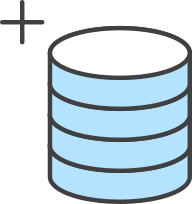
\includegraphics[width=0.4\linewidth]{figures/gitcreate}
		\end{figure}	
		\begin{figure}
			\centering			
			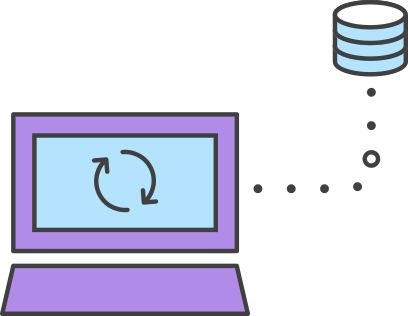
\includegraphics[width=0.6\linewidth]{figures/gitsync}
		\end{figure}
		\begin{figure}
			\centering			
			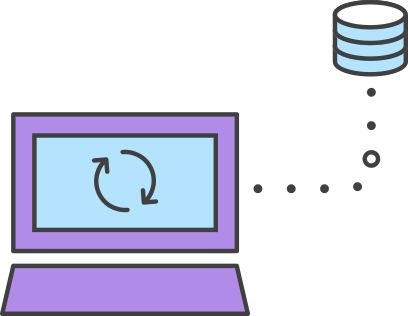
\includegraphics[width=0.6\linewidth]{figures/gitsync}
		\end{figure}
	\end{column}
\end{columns}

\end{frame}

\subsection{Fazendo alterações}
% ----------------- NOVO SLIDE --------------------------------	
\begin{frame}[fragile]{Git Workflow}
\framesubtitle{Fazendo alterações}
	\begin{block}{Lista os arquivo novos ou modificados}		
		\begin{verbatim}
		$ git status
		\end{verbatim}
	\end{block}			

	\begin{block}{Prepara o arquivo para o versionamento | \textit{staging area}}		
		\begin{verbatim}
		$ git add [nome do arquivo]
		\end{verbatim}
	\end{block}
	
	\begin{block}{Mostra a diferença entre os arquivos}		
		\begin{verbatim}
		$ git diff ou $ git diff --staged		
		\end{verbatim}
	\end{block}		

	\begin{block}{Grava modificações no histórico de versão}		
		\begin{verbatim}
		$ git commit -m "[mensagem descritiva]"
		\end{verbatim}
	\end{block}		

	\begin{block}{Verifique o histórico de versões}		
		\begin{verbatim}
		$ git log
		\end{verbatim}
	\end{block}					
\end{frame}

% ----------------- NOVO SLIDE --------------------------------	
\begin{frame}[fragile]{Git Workflow}
\framesubtitle{Fazendo alterações | Entendendo as áreas de trabalho}

	\begin{figure}
		\centering			
		
\includegraphics[width=0.6\linewidth]{figures/treesv2}
	\end{figure}	
	
	\begin{itemize}		
		\small
		\item[$\checkmark$] Seus repositórios locais consistem em três "árvores" mantidas pelo git. 
		\item[$\checkmark$] Working Directory - contém os arquivos vigentes.
		\item[$\checkmark$] Index (Stage) - funciona como uma área temporária
		\item[$\checkmark$] HEAD - aponta para o último commit (confirmação) que você fez. 
	\end{itemize}

\end{frame}

\subsection{Exemplo - primeiros passos}
% ----------------- NOVO SLIDE --------------------------------	
\begin{frame}[fragile]{Git Workflow}
\framesubtitle{Exemplo prático | Primeiros passos com git}

	\begin{enumerate}
		\item crie um novo diretório e prepare [ou clone] o repositório
		\begin{verbatim}
			$ git init
		\end{verbatim}
		
		\item adicione [ou modifique] os arquivos de trabalho		
		
		\item verifique os arquivos alterados		
		\begin{verbatim}
			$ git status 
		\end{verbatim}
		
		\item adicione os arquivos desejados a \textit{staging area} 
		\begin{verbatim}
			$ git add
		\end{verbatim}
		
		\begin{itemize}
			\item + alterações? | verifique  |  \textit{staging area}
			\begin{verbatim}
				$ git status | $ git diff | $ git add
			\end{verbatim}
		\end{itemize}
	
		\item grave as modificações no histórico de versão
		\begin{verbatim}
			$ git commit -m "[mensagem descritiva]"
		\end{verbatim}
		
		\item verifique o histórico de versões
		\begin{verbatim}
		$ git log"
		\end{verbatim}
	\end{enumerate}

\end{frame}


\subsection{Colaborando e Sincronizando}
% ----------------- NOVO SLIDE --------------------------------	
\begin{frame}[fragile]{Git Workflow}
\framesubtitle{Colaborando e Sincronizando  | Criando as contas no github e gitlab}

\vfill
\begin{columns}[t]
	\begin{column}{.5\textwidth}
		\begin{figure}
			\centering
			\includegraphics[width=0.7\linewidth]{figures/Github_logo}
			\caption*{	\href{https://github.com/}{\color{blue}Github}}
		\end{figure}
	\end{column}
	\begin{column}{.5\textwidth}
		\begin{figure}
			\centering
			
\includegraphics[width=0.7\linewidth]{figures/GitLab_logo}
			\caption*{\href{https://gitlab.com/}{\color{blue}Gitlab}}
		\end{figure}		
	\end{column}
\end{columns}
\vfill
\begin{exampleblock}{Após criar a conta...}
 crie um novo repositório
\end{exampleblock}
\vfill
\end{frame}

% ----------------- NOVO SLIDE --------------------------------	
\begin{frame}[fragile]{Git Workflow}
\framesubtitle{Colaborando e Sincronizando  | Configurando o caminho }

\begin{figure}
	\centering			
	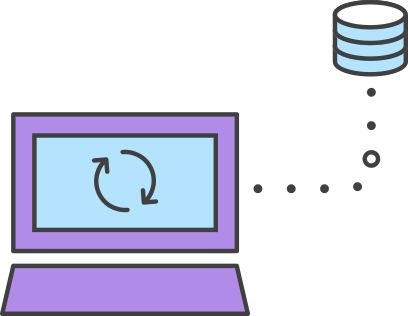
\includegraphics[width=0.2\linewidth]{figures/gitsync}
\end{figure}

\begin{block}{Define o caminho até um repositório na nuvem}		
	\begin{verbatim}
	$ git remote add <origin> [url]
	\end{verbatim}
\end{block}

\begin{block}{verifique o caminho}		
	\begin{verbatim}	
	$ git remote -v 
	\end{verbatim}
\end{block}

\end{frame}


% ----------------- NOVO SLIDE --------------------------------	
\begin{frame}[fragile]{Git Workflow}
\framesubtitle{Colaborando e Sincronizando  | repo nuvem = repo local }

\begin{figure}
	\centering			
	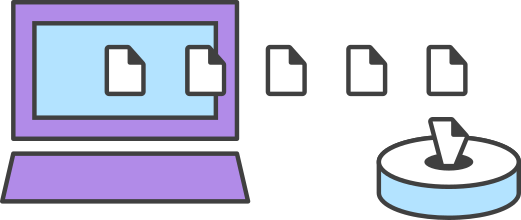
\includegraphics[width=0.2\linewidth]{figures/gitclone}
\end{figure}

\begin{block}{Sincronize o histórico de versão na nuvem com o repositório local}		
	\begin{verbatim}
	$ git fetch <origin>
	\end{verbatim}
\end{block}			

\begin{block}{Verifique o histórico de versão sincronizado}		
	\begin{verbatim}	
	$ git log <origin>/master
	\end{verbatim}
\end{block}

\begin{block}{Combine os repositórios}		
	\begin{verbatim}	
	$ git merge <origin>/master
	\end{verbatim}
\end{block}

\end{frame}


% ----------------- NOVO SLIDE --------------------------------	
\begin{frame}[fragile]{Git Workflow}
\framesubtitle{Colaborando e Sincronizando  | repo nuvem = repo local }
\begin{figure}
	\centering			
	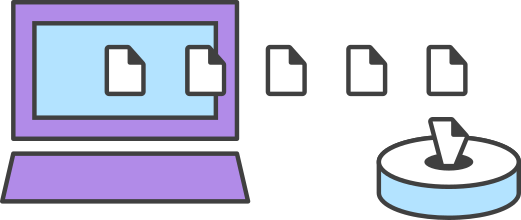
\includegraphics[width=0.2\linewidth]{figures/gitclone}
\end{figure}

\begin{exampleblock}{Sincronização e combinação de uma vez}
	\begin{verbatim}
		$ git pull <origin>
	\end{verbatim}
\end{exampleblock}
{\tiny$ \star $Se tiver certeza que a sincronização e combinação pode ser feita, agilize o processo com esse comando único}

\begin{block}{Sincronize o histórico de versão local com o repositório na nuvem}		
	\begin{verbatim}
	$ git push <origin> master
	\end{verbatim}
\end{block}			


\end{frame}

\subsection{Exemplo - primeiros passos}
% ----------------- NOVO SLIDE --------------------------------	
\begin{frame}[fragile]{Git Workflow}
\framesubtitle{Exemplo prático | Sincronizando com a nuvem}

\begin{enumerate}
	\item Adicione o caminho do repositório na nuvem e confirme o caminho
	\begin{verbatim}
	$ git remote add <origin> [url]
	$ git remote -v
	\end{verbatim}
	
	\item Sincronize o repositório da nuvem com o repositório local
	\begin{verbatim}
		$ git fetch <origin>
		$ git log <origin>/master
		$ git merge <origin>/master
	\end{verbatim}
	ou 
	\begin{verbatim}
		$ git pull <origin>
	\end{verbatim}
	\item verifique os arquivos alterados		
	\begin{verbatim}
	$ git status 
	\end{verbatim}
	
	\item Faça alterações no seu repositório local
	\item grave as modificações no histórico de versão e verifique
	\item Sincronize o histórico de versão local com o repositório na nuvem
	
\end{enumerate}

\end{frame}

\section{Git Workflow Avançado [não finalizado]}

% ----------------- NOVO SLIDE --------------------------------	
\begin{frame}{}
\tiny
\tableofcontents[current]
\end{frame}

\subsection{Branches}
%% ----------------- NOVO SLIDE --------------------------------	
%\begin{frame}[fragile]{Git Workflow}
%\framesubtitle{Branches | Ramificações}
%	\begin{figure}
%		\centering			
%		
\includegraphics[width=0.4\linewidth]{figures/branchesv2}
%	\end{figure}
%
%	\begin{block}{Lista todos os branches locais}		
%		\begin{verbatim}
%			$ git branch
%		\end{verbatim}
%	\end{block}			
%
%	\begin{block}{Cria um novo branch}		
%		\begin{verbatim}
%			$ git branch [nome-do-branch]
%		\end{verbatim}
%	\end{block}			
%
%	\begin{block}{Muda para o branch específico e atualiza o diretório}		
%		\begin{verbatim}
%			$ git checkout [nome-do-branch]
%		\end{verbatim}
%	\end{block}			
%
%	\begin{block}{Combina o histórico do branch especifíco com o atual}		
%		\begin{verbatim}
%			$ git merge [nome-do-branch]
%		\end{verbatim}
%	\end{block}			
%
%\end{frame}

\subsection{Fork}

\subsection{Trabalhando em equipe}


\section{Links uteis e referências}
% ----------------- NOVO SLIDE --------------------------------	
\begin{frame}{Links úteis e referências}

	\begin{itemize}		
	\item[$\blacksquare$] \href{https://guides.github.com/introduction/git-handbook/}{\color{blue}Git hub handbook}
	\item[$\blacksquare$] \href{https://help.github.com/articles/github-glossary/}{\color{blue} Git hub glossary}
	\item[$\blacksquare$] \href{https://github.com/pbs-assess/git-course}{\color{blue} GitHub by Chris Grandin and Andrew Edwards}
	\item[$\blacksquare$] \href{https://try.github.io/}{\color{blue} Resources to learn Git}
	\item[$\blacksquare$] \href{https://www.atlassian.com/git}{\color{blue} Atlassian} 			
	\item[$\blacksquare$]  \href{http://rogerdudler.github.io/git-guide/index.pt_BR.html}{\color{blue} git - guia prático} 			
	\end{itemize}
	
%	\bibliography{../references}
\end{frame}

\end{document}